\scanpage{27}
\begingroup\makeatletter\tagsleft@true\makeatother
\margin{\begin{tikzpicture}
\node[inner sep=1pt,align=left,text width=.93\marginparwidth] (titre) {structure filtrée sur DR et comparaison avec Betti, Hdg...};
\draw (titre.north west) -- (titre.south west) -- (titre.south east);
\end{tikzpicture}}

Soit $k\unsure{\mathrel{\tikz[x=.58em,y=.58em,baseline=0pt,line cap=round]{\draw (.87,.44) .. controls (.60,.70) and (-.03,.34) .. (.04,.17) .. controls (.12,.04) and (.78,.09) .. (1.20,.02); \draw (1.23,.14) -- (1.14,.80) .. controls (1.15,.96) and (.92,.79) .. (.99,1.00) .. controls (1.01,1.08) and (1.05,1.12) .. (1.09,1.13);}}|\subset^{\iota}|\subset}\mathbb{C}$, considérons une catégor. de motifs \inserted{sur $k$,} de type fini \deleted{\unsure{soit}}, soit $\mathcal{M}$. Il y a deux foncteurs fibres naturels,
\[
T_{\mathrm{DR}}:\mathcal{M}\relbar\operatorname{Mod}f(k)\tag*{(1)}
\]
\diagram{\begin{minipage}{\linewidth}
\[
\begin{tikzcd}[ampersand replacement=\&,column sep=1.2em]
T_{B\unsure{\mathrm{dg}|\mathrm{Hdg}|\mathrm{tg}}}:\mathcal{M}\arrow[r]\&
\deleted{\operatorname{Mod}f(\unsure{\mathbb Q|Q})}\ \mathrm{Str.}\ \mathrm{Hodge}\arrow[r]\&
\operatorname{Mod}f(\mathbb Q),
\end{tikzcd}\tag*{(2)}
\]
\end{minipage}}
le deuxième dépendant de l'imm. $k\subset\mathbb{C}$. Le premier a une structure de filtration. De plus, on a un isom canonique
\[
\varphi:T_B\otimes_{\mathbb Q}\mathbb C\xrightarrow{\sim}T_{\mathrm{DR}}\otimes_k\mathbb C\tag*{(3)}
\]
\inserted{compatible aux filtrations des 2 \unsure{mbres|mbrs}}

Soit $G$ gpe des Aut. de $T_B$. Comparant $T_{\mathrm{DR}}$ et $T_B\otimes_{\mathbb Q}k$, on trouve un torseur à droite
\[
P=\unsure{\underline{\operatorname{Isom}}|\underrightarrow{\operatorname{Isom}}}_{\otimes}(T_B\otimes_{\mathbb Q}k,T_{\mathrm{DR}})\tag*{(4)}
\]
sous $G_k$, qui permet de récupérer le foncteur $T_{\mathrm{DR}}$ comme
\[
T_{\mathrm{DR}}=\deleted{T_B\otimes}\ P\overset{G_k}{\times}(T_B\otimes_{\mathbb Q}k).\tag*{(5)}
\]
De plus, \deleted{\unsure{on a un isom.}} l'isom (3) définit un élément canonique
\[
\varphi\in P(\mathbb C)
\]
\margin{\begin{tikzpicture}
\node[inner sep=1pt,align=left,text width=.91\marginparwidth] (note) {La connaissance de $G,P,\varphi$ permet de récupérer ess. $\mathcal M$ avec (1) (2) et (3)};
\draw ([xshift=1pt]note.north west) -- ([xshift=-3pt]note.south west);
\end{tikzpicture}}% slanted

Pour récupérer la structure filtrée sur $T_{\mathrm{DR}}$, \deleted{et} donc la structure de Hodge sur $T_B$ i.e la bigraduation sur $T_B\otimes_{\mathbb Q}C$, il convient d'introduire
\[
T_{\mathrm{Hdg}}\unsure{\in|\mathord{:}}\mathcal M\longrightarrow\operatorname{Mod}\deleted{\unsure{\mathrm{Bi}|\mathrm B}}\mathrm{grad}\,f(k),\qquad T_{\mathrm{Hdg}}=\operatorname{gr}^{*}T_{\mathrm{DR}}.\tag*{(6)}
\]
\inserted{Soit} \deleted{et les deux \unsure{groupes|grpes} de} \deleted{Lie}
\[
\deleted{\unsure{H|K}}\ G'_k=P\overset{G_k}{\times}G_k=\operatorname{ad}(P)\simeq\underline{\operatorname{Aut}}_{\otimes}(T_{\mathrm{DR}})\tag*{(7)}
\]
\deleted{\unsure{Ainsi|Alors}} et
\[
\begin{aligned}
H'\subset G'_k\qquad &\text{ss grpe des $\otimes$-Aut de $T_{\mathrm{DR}}$ respectant}\\
&\text{la filtration et qui induisent l'}\\
&\text{identité sur le gradué associé.}
\end{aligned}\tag*{(8)}
\]
\endgroup
% archive sheet number: 26
